\section{Experimental Setup}

\subsection{Simulator and Task}

Experiments use an AutoTrans-like suspended-payload UAV stack in simulation.
The task is to transport a cable-suspended payload to a target under a strong
wind setting while preserving arrival behavior, bounded tracking, and stable
post-arrival hold behavior. The evaluated scenarios focus on Trials 4, 5, and
6, which were selected in the Stage 4 workflow because they expose
strong-wind failures and method differences.

\subsection{Strict-Valid Metric}

The paper-facing metric is strict-valid count over repeated runs. A strict
valid run must satisfy the Stage 4 validity checks used throughout the
protocol-split evaluation. We report strict-valid counts rather than only raw
suggested validity because warning-style diagnostics and invalid-only failure
groups are needed to interpret failure modes.

\subsection{Protocol Definitions}

We evaluate two protocols separately. The single-goal mission protocol uses
\texttt{goal\_repeat=1}, meaning the goal is published once. The goal-reissue
stress protocol uses \texttt{goal\_repeat=10}, repeatedly republishing the
same goal and stressing reference-update, post-arrival, and repeated-command
behavior.

\begin{figure}[t]
  \centering
  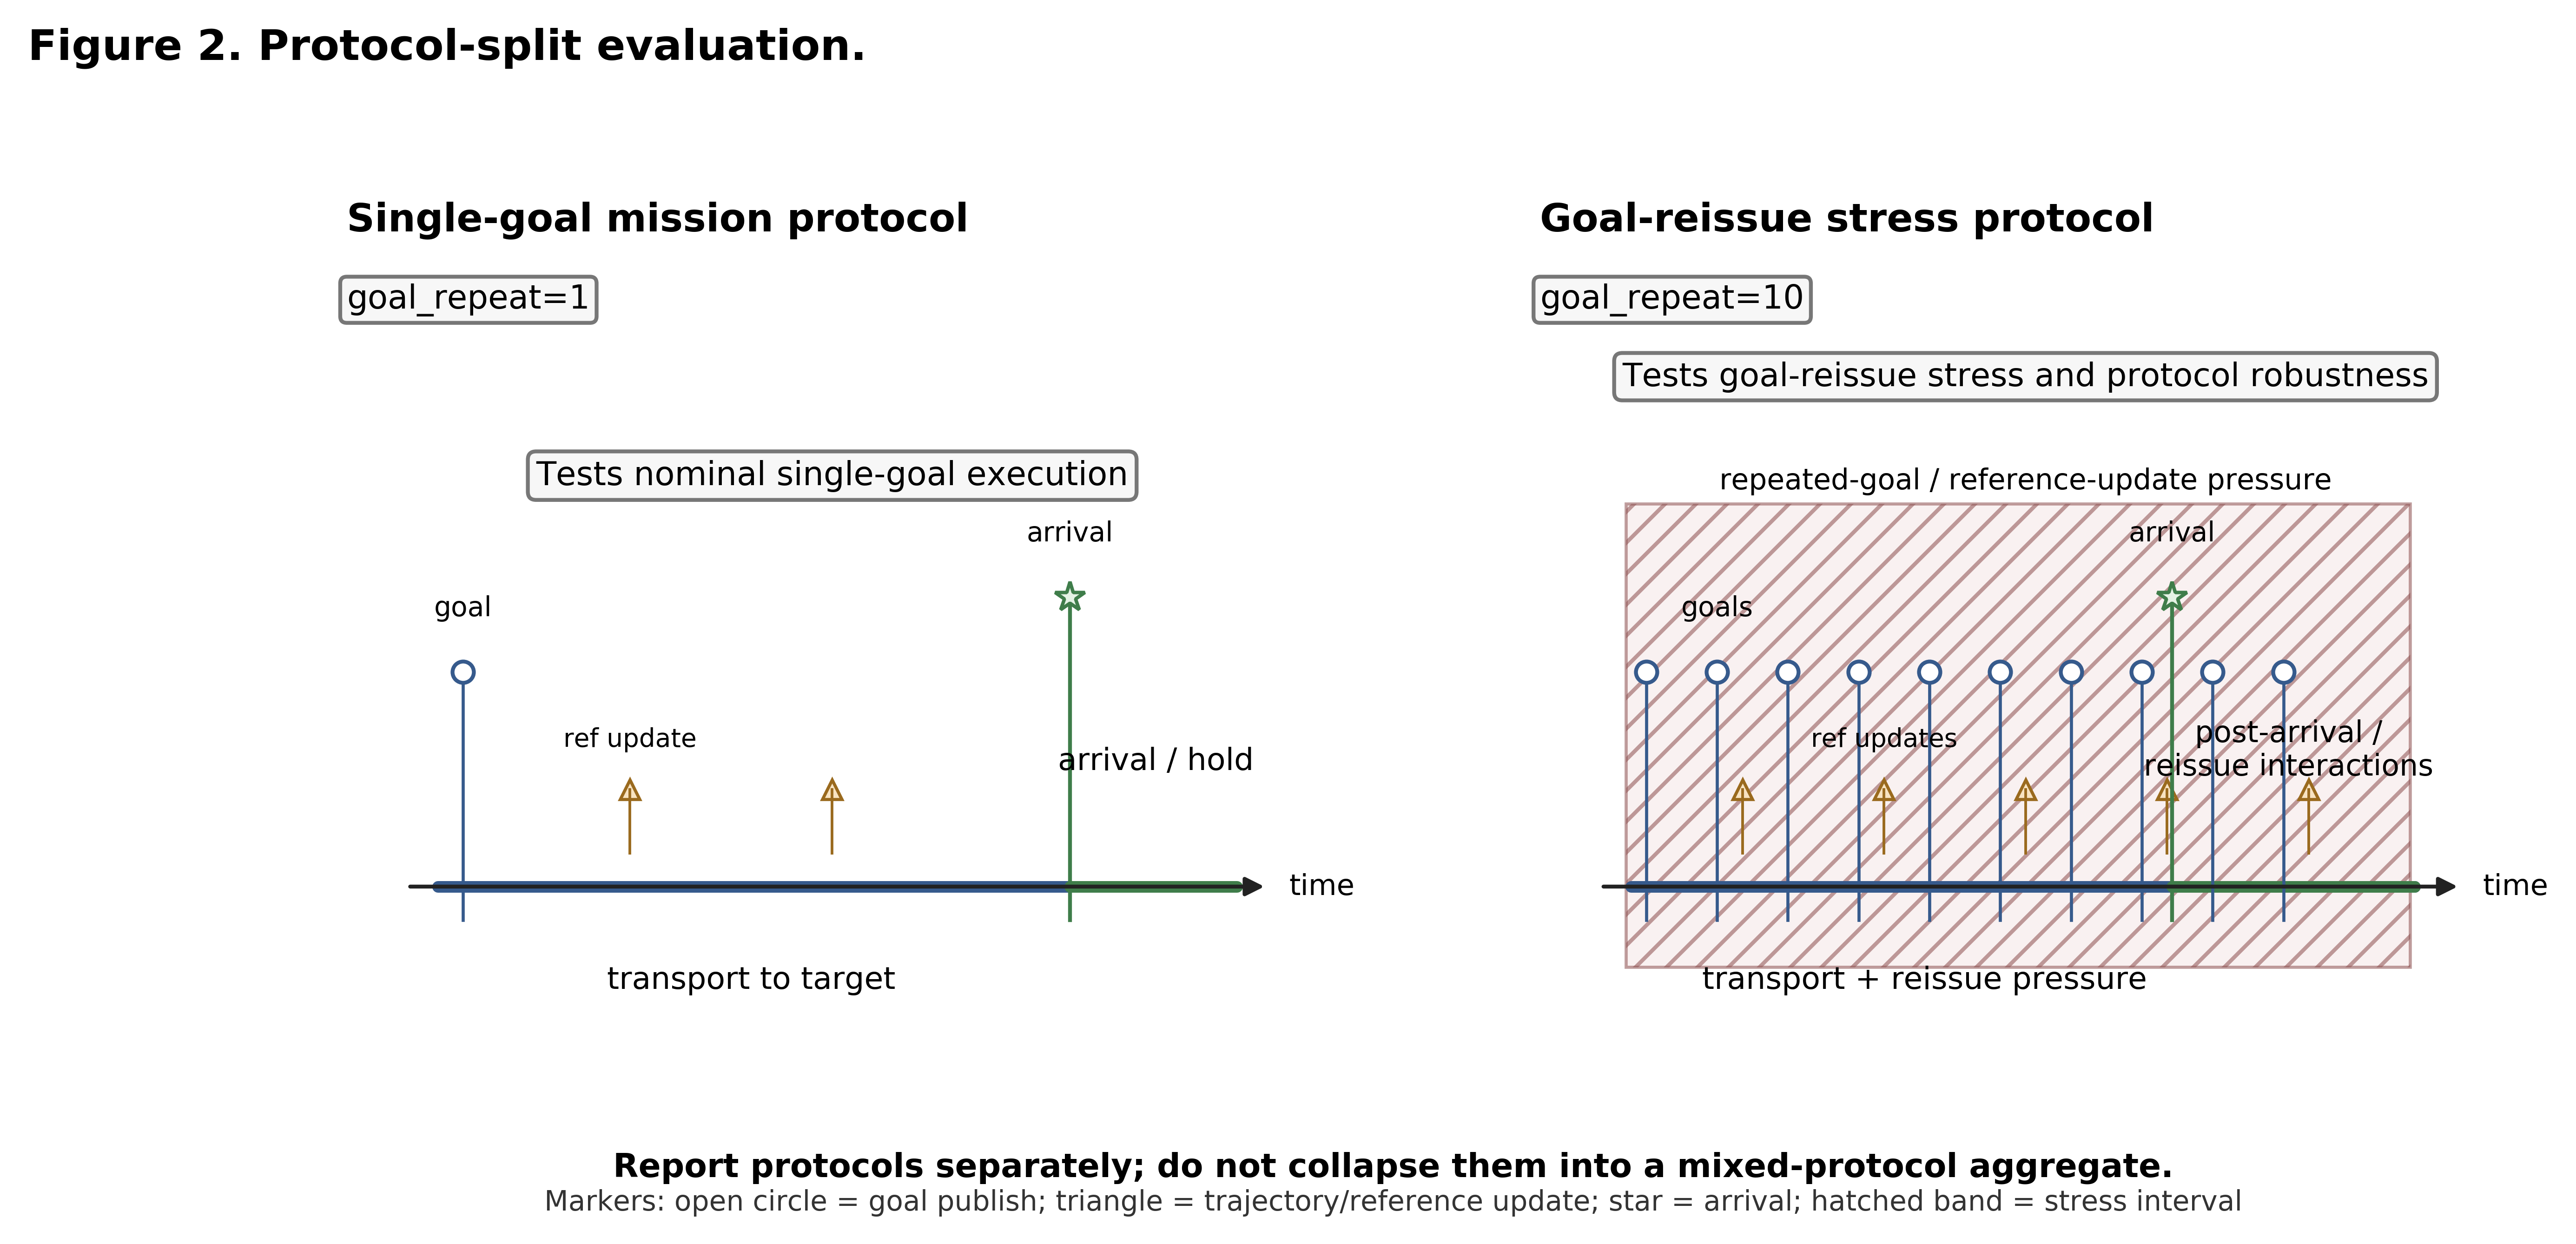
\includegraphics[width=\linewidth]{figures/fig2_protocol_split.png}
  \caption{Protocol-split evaluation. The single-goal mission protocol uses
  one goal publish, whereas the goal-reissue stress protocol repeatedly
  republishes the same goal. Results are reported separately to avoid a
  mixed-protocol aggregate.}
  \label{fig:protocol_split}
\end{figure}

\subsection{Compared Methods}

The complete cross-protocol table includes \texttt{original},
\texttt{fixed\_s085}, \texttt{windlevel\_s085}, \texttt{fixed\_s080},
\texttt{risk\_adapter\_v1}, and \texttt{risk\_adapter\_v21}.
\texttt{risk\_adapter\_v2} has a single-goal result but lacks the matching
stress result, so it is treated as a supplementary single-protocol-only note
rather than a main balanced-ranking entry.

\subsection{Repeated-Run Design and Diagnostic Logging}

Each complete method/protocol combination is evaluated over 30 repeated runs
across Trials 4, 5, and 6. Diagnostic logs support strict-valid classification,
invalid-only failure grouping, command-scale inspection, risk-score inspection,
arrival timing, NaN timing, and representative trace analysis. These diagnostic
views are used to interpret failures, not to replace strict-valid count as the
main paper metric.
